\section{Wechseltromkreise}
\Large 
\begin{frame}
    \centering
    \visible<2->{
    \begin{tikzpicture}
        \path[very thick, -{Latex}] (0, 0) edge (10, 0) (0, -1) edge (0, 3);
        \node[right] at (10, 0) {$t$};
        \draw[thick, red] (0, 0) sin (1, 1) cos (2, 0)
            sin (3, -1) cos (4, 0)
            sin (5, +1) cos (6, 0)
            sin (7, -1) cos (8, 0);
    \end{tikzpicture}
    }
    \\
    \visible<3>{
        \[ A(t) = \hat A\sin(\omega t + \phi) \]
    }
\end{frame}

\section{Die Bauteile}
\begin{frame}
    \centering\Huge
    \visible<1->{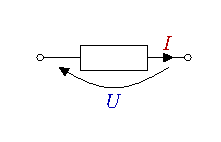
\includegraphics[width=.5\textwidth]{../script/kBR.pdf}}
    \visible<2->{
    \parbox[b]{.4\textwidth}{
        $$U = R\cdot I$$
        \vspace{16mm}
    }}
    \vspace{-1cm}  % caught in the act
    \visible<3>{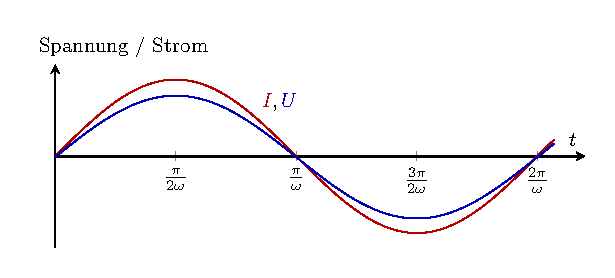
\includegraphics[width=.7\textwidth]{../script/kPR.pdf}}
\end{frame}
\begin{frame}
    \centering\huge
    \visible<1->{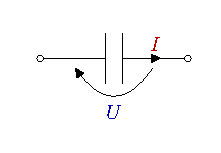
\includegraphics[width=.5\textwidth]{../script/kBC.pdf}}
    \visible<2->{
    \parbox[b]{.4\textwidth}{
        $$I = C\dot U$$
        \vspace{16mm}
    }}
    \visible<3>{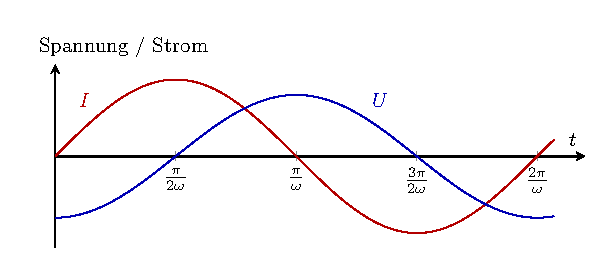
\includegraphics[width=.7\textwidth]{../script/kPC.pdf}}
\end{frame}
\begin{frame}
    \centering\huge
    \visible<1->{\includegraphics[width=.5\textwidth]{../script/kBL.pdf}}
    \visible<2->{
    \parbox[b]{.4\textwidth}{
        $$U = L\dot I$$
        \vspace{16mm}
    }}
    \vspace{-1cm}  % caught in the act
    \visible<3>{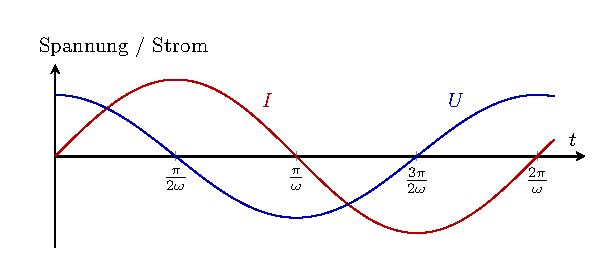
\includegraphics[width=.7\textwidth]{../script/kPL.pdf}}
\end{frame}
